\documentclass{beamer}
\usetheme{Berlin}
\usepackage[T1]{fontenc}
\usepackage{minted}
\usepackage{etoolbox}
\usepackage{setspace}
\usepackage{bussproofs}
\usepackage{amsmath}
\usepackage{amsthm}
\usepackage{amssymb}
\usepackage{amsxtra}
\usepackage{csquotes}
\usepackage[croatian]{babel}
\DeclareRobustCommand{\VDash}{\mathrel{||}\joinrel\Relbar}

\BeforeBeginEnvironment{minted}{\begin{spacing}{1.0}}
\AfterEndEnvironment{minted}{\end{spacing}}
\AfterEndEnvironment{minted}{\vspace{0pt}}

\DeclareUnicodeCharacter{22A8}{\(\vDash\)}
\DeclareUnicodeCharacter{22A2}{\(\vdash\)}
\DeclareUnicodeCharacter{2286}{\(\subseteq\)}
\DeclareUnicodeCharacter{22AB}{\(\VDash\)}
\DeclareUnicodeCharacter{2291}{\(\sqsubseteq\)}
\DeclareUnicodeCharacter{03A3}{\(\Sigma\)}
\DeclareUnicodeCharacter{03C1}{\(\rho\)}
\DeclareUnicodeCharacter{03C6}{\(\varphi\)}
\DeclareUnicodeCharacter{03A6}{\(\Phi\)}
\DeclareUnicodeCharacter{03B1}{\(\alpha\)}
\DeclareUnicodeCharacter{03C9}{\(\omega\)}
\DeclareUnicodeCharacter{0393}{\(\Gamma\)}
\DeclareUnicodeCharacter{0394}{\(\Delta\)}
\DeclareUnicodeCharacter{03C8}{\(\psi\)}

\title{Primjene Coq alata za dokazivanje u matematici i računarstvu}
\subtitle{Logika prvog reda s induktivnim definicijama}
\author{Miho Hren}
\institute{Mentori: Vedran Čačić, Marko Doko \(+\) Ante Đerek\\
  Fakultet Elektrotehnike i Računarstva}
\date{2023./2024.}

\setbeamertemplate{headline}{}
\setbeamertemplate{footline}[frame number]
\setbeamertemplate{navigation symbols}{}


\begin{document}
\begin{frame}
  \titlepage{}
\end{frame}

\begin{frame}
  \frametitle{Proces}
  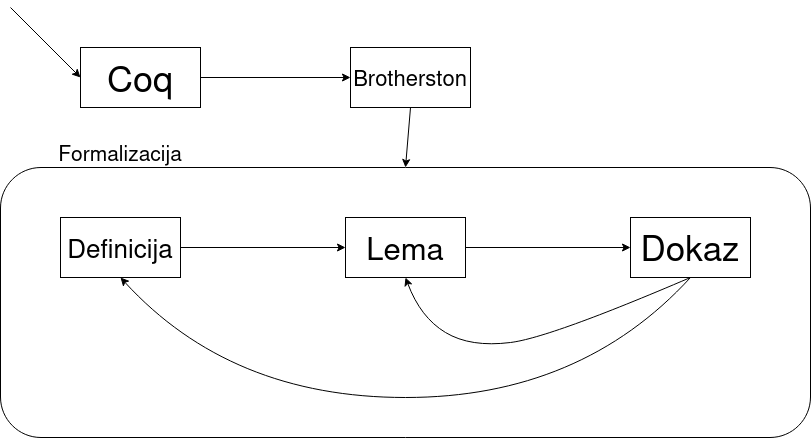
\includegraphics[width=\textwidth]{diplomskiproces.png}
\end{frame}

\begin{frame}[fragile]
  \frametitle{Sintaksa: signatura}
\begin{minted}{coq}
Structure signature := {
    FuncS : Set;
    fun_ar : FuncS -> nat;
    PredS : Set;
    pred_ar : PredS -> nat;
    IndPredS : Set;
    indpred_ar : IndPredS -> nat;
  }.

Context {Σ : signature}.
\end{minted}
  \begin{block}{Peanova signatura}
      \[
    \sigma_{\mathit{PA}} = \{ \{ o^{0}, s^{1}, +^{2}, \cdot^{2} \},
    \{=^{2}\}, \{\mathit{Nat}^{1}, \mathit{Even}^{1}, \mathit{Odd}^{1}\}\}
  \]
  \end{block}
\end{frame}

\begin{frame}[fragile]
  \frametitle{Sintaksa: termi, formule}
\begin{minted}{coq}
Inductive term  : Set :=
| var_term : var -> term 
| TFunc : forall (f : FuncS Σ),
    vec term (fun_ar f) -> term.

Inductive formula : Set :=
| FPred (P : PredS Σ)
    : vec (term Σ) (pred_ar P) -> formula 
| FIndPred (P : IndPredS Σ)
    : vec (term Σ) (indpred_ar P) -> formula 
| FNeg : formula -> formula 
| FImp : formula -> formula -> formula 
| FAll : formula -> formula.
\end{minted}

\end{frame}

\begin{frame}[fragile]
  \frametitle{Sintaksa: produkcije}
  \begin{huge}
    \begin{prooftree}
      \AxiomC{\(  Q_{1}\mathbf{u}_{1}  \ldots   Q_{n}\mathbf{u}_{n}  \)}
      \AxiomC{\(  P_{1}\mathbf{v}_{1}  \ldots   P_{m}\mathbf{v}_{m}  \)}
      \BinaryInfC{\(P\mathbf{t}\)}
    \end{prooftree}
  \end{huge}
  \begin{small}
\begin{minted}{coq}
Record production :=
  mkProd {
      preds
        : list {P: PredS Σ & vec (term Σ) (pred_ar P)};
      indpreds
        : list {P: IndPredS Σ & vec (term Σ) (indpred_ar P)};
      indcons : IndPredS Σ;
      indargs : vec (term Σ) (indpred_ar indcons);
    }.
\end{minted}
  \end{small}
\end{frame}

\begin{frame}
  \begin{block}{Biti prirodan broj.}
    \begin{minipage}[t]{0.48\linewidth}
      \begin{prooftree}
        \AxiomC{}
        % \RightLabel{(\texttt{PA\_prod\_N\_zero})}
        \UnaryInfC{\( \mathit{Nat}(o) \)}
      \end{prooftree}
    \end{minipage}
    \begin{minipage}[t]{0.48\linewidth}
      \begin{prooftree}
        \AxiomC{\( \mathit{Nat}(x) \)}
        % \RightLabel{(\texttt{PA\_prod\_N\_succ})}
        \UnaryInfC{\( \mathit{Nat}(s(x)) \)}
      \end{prooftree}
    \end{minipage}
  \end{block}
  \begin{block}{Biti paran, odnosno neparan broj.}
    \begin{minipage}[t]{0.31\linewidth}
      \begin{prooftree}
        \AxiomC{}
        % \RightLabel{(\texttt{PA\_prod\_E\_zero})}
        \UnaryInfC{\( \mathit{Even}(o) \)}
      \end{prooftree}
    \end{minipage}
    \begin{minipage}[t]{0.31\linewidth}
      \begin{prooftree}
        \AxiomC{\( \mathit{Odd}(x) \)}
        % \RightLabel{(\texttt{PA\_prod\_E\_succ})}
        \UnaryInfC{\( \mathit{Even}(s(x)) \)}
      \end{prooftree}
    \end{minipage}
    \begin{minipage}[t]{0.31\linewidth}
      \begin{prooftree}
        \AxiomC{\( \mathit{Even}(x) \)}
        % \RightLabel{(\texttt{PA\_prod\_O\_succ})}
        \UnaryInfC{\( \mathit{Odd}(s(x)) \)}
      \end{prooftree}
    \end{minipage}
  \end{block}
\end{frame}

\begin{frame}[fragile]
  \frametitle{Semantika: struktura, okolina}
\begin{minted}{coq}
Structure structure := {
    domain :> Set;
    interpF (f : FuncS Σ)
        : vec domain (fun_ar f) -> domain;
    interpP (P : PredS Σ)
        : vec domain (pred_ar P) -> Prop;
    interpIP (P : IndPredS Σ)
        : vec domain (indpred_ar P) -> Prop;
  }.

Definition env := var -> M.
\end{minted}
  \begin{block}{Standardna Peanova struktura}
    \[
      M_{\mathit{PA}} = (\mathbb{N}, 0, S, +, \cdot, =, \mathbb{N}, \mathbb{E}, \mathbb{O})
    \]
  \end{block}
\end{frame}

\begin{frame}[fragile]
  \frametitle{Semantika: istinitost formule}
\begin{minted}{coq}
Fixpoint Sat (ρ : env M) (F : formula Σ) : Prop :=
  match F with
  | FPred P args => interpP P (V.map (eval ρ) args)
  | FIndPred P args => interpIP P (V.map (eval ρ) args)
  | FNeg G => ~ Sat ρ G
  | FImp F G => Sat ρ F -> Sat ρ G
  | FAll G => forall d, Sat (d .: ρ) G
  end.
\end{minted}
  \begin{block}{Primjer}
    \[
      (M_{\mathit{PA}}, \rho) \vDash \forall x, \mathit{Nat}(x) \rightarrow \mathit{Even}(x) \lor \mathit{Odd}(x)
    \]
  \end{block}
\end{frame}

\begin{frame}[fragile]
  \frametitle{Semantika: produkcije}
\begin{minted}{coq}
Definition InterpInd :=
    forall P : IndPredS Σ, vec M (indpred_ar P) -> Prop.

Fixpoint φ_Φ_n (α : nat) : InterpInd :=
  match α with
  | 0 => fun _ _ => False
  | S α => φ_Φ (φ_Φ_n α)
  end.

Definition φ_Φ_ω : InterpInd :=
    fun P v => exists α, φ_Φ_n α P v.
\end{minted}
\end{frame}

\begin{frame}[fragile]
  \frametitle{Semantika: standardni modeli}
\begin{minted}{coq}
Lemma φ_Φ_ω_least_prefixed : least prefixed φ_Φ_ω.

Definition standard_model
  (Φ: IndDefSet Σ)
  (M : structure Σ)
  : Prop :=
    forall (P : IndPredS Σ) ts,
      interpIP P ts <-> φ_Φ_ω Φ M P ts.
\end{minted}
\end{frame}

\begin{frame}[fragile,fragile]
  \frametitle{Sekvente}
\begin{minted}{coq}
Inductive sequent : Set :=
| mkSeq (Γ Δ : list (formula Σ)).
\end{minted}
  \[
    \Gamma \vdash \Delta
  \]

\begin{minted}{coq}
Definition Sat_sequent (s : sequent) : Prop :=
  let '(Γ ⊢ Δ) := s in            
  forall (M : structure Σ),
      standard_model Φ M -> forall (ρ : env M),
        (forall φ, In φ Γ -> ρ ⊨ φ) ->
        exists ψ, In ψ Δ /\ ρ ⊨ ψ.
\end{minted}
  \[
    \Gamma \VDash \Delta
  \]
\end{frame}

\begin{frame}
  \frametitle{Sistem sekvenata: \enquote{obična} pravila izvoda}
  \begin{small}
    \begin{block}{}
      \begin{minipage}[t]{0.33\linewidth}
        \begin{prooftree}
          \AxiomC{\(\Gamma \cap \Delta \not = \varnothing \)}
          \RightLabel{\( \mathit{ (Ax) } \)}
          \UnaryInfC{\( \Gamma \vdash \Delta \)}
        \end{prooftree}
      \end{minipage}
      \begin{minipage}[t]{0.48\linewidth}
        \begin{prooftree}
          \AxiomC{\(\Gamma^{\prime} \vdash \Delta^{\prime}\)}
          \AxiomC{\(\Gamma^{\prime} \subseteq \Gamma\)}
          \AxiomC{\(\Delta^{\prime} \subseteq \Delta\)}
          \RightLabel{\( \mathit{ (Wk) } \)}
          \TrinaryInfC{\(\Gamma \subseteq \Delta\)}
        \end{prooftree}
      \end{minipage}
      \begin{minipage}[t]{0.48\linewidth}
        \begin{prooftree}
          \AxiomC{\( \Gamma \vdash \varphi, \Delta\)}
          \AxiomC{\( \varphi, \Gamma \vdash \Delta \)}
          \RightLabel{\( \mathit{ (Cut) } \)}
          \BinaryInfC{\( \Gamma \vdash \Delta \)}
        \end{prooftree}
      \end{minipage}
      \begin{minipage}[t]{0.48\linewidth}
        \begin{prooftree}
          \AxiomC{\( \Gamma \vdash \Delta \)}
          \RightLabel{\( \mathit{ (Subst) } \)}
          \UnaryInfC{\( \Gamma[\sigma] \vdash \Delta[\sigma] \)}
        \end{prooftree}
      \end{minipage}
    \end{block}
    \begin{block}{}
      \begin{minipage}[t]{0.48\linewidth}
        \begin{prooftree}
          \AxiomC{\( \Gamma \vdash \varphi, \Delta \)}
          \RightLabel{\( \mathit{ (NegL) } \)}
          \UnaryInfC{\( \neg \varphi, \Gamma \vdash \Delta \)}
        \end{prooftree}
      \end{minipage}
      \begin{minipage}[t]{0.48\linewidth}
        \begin{prooftree}
          \AxiomC{\( \varphi, \Gamma \vdash \Delta \)}
          \RightLabel{\( \mathit{ (NegR) } \)}
          \UnaryInfC{\( \Gamma \vdash \neg \varphi, \Delta \)}
        \end{prooftree}
      \end{minipage}
      \begin{minipage}[t]{0.48\linewidth}
        \begin{prooftree}
          \AxiomC{\( \Gamma \vdash \varphi, \Delta \)}
          \AxiomC{\( \psi, \Gamma \vdash \Delta \)}
          \RightLabel{\( \mathit{ (ImpL) } \)}
          \BinaryInfC{\( \varphi \rightarrow \psi, \Gamma \vdash \Delta \)}
        \end{prooftree}
      \end{minipage}
      \begin{minipage}[t]{0.48\linewidth}
        \begin{prooftree}
          \AxiomC{\( \varphi, \Gamma \vdash \psi, \Delta \)}
          \RightLabel{\( \mathit{ (ImpR) } \)}
          \UnaryInfC{\( \Gamma \vdash \varphi \rightarrow \psi, \Delta \)}
        \end{prooftree}
      \end{minipage}
    \end{block}
    \begin{block}{}
      \begin{minipage}[t]{0.48\linewidth}
        \begin{prooftree}
          \AxiomC{\( \varphi[t \cdot \sigma_{\mathit{id}}], \Gamma \vdash \Delta \)}
          \RightLabel{\( \mathit{ (AllL) } \)}
          \UnaryInfC{\( \forall\varphi, \Gamma \vdash \Delta \)}
        \end{prooftree}
      \end{minipage}
      \begin{minipage}[t]{0.48\linewidth}
        \begin{prooftree}
          \AxiomC{\( \Gamma^{\uparrow} \vdash \varphi, \Delta^{\uparrow}\)}
          \RightLabel{\( \mathit{ (AllR) } \)}
          \UnaryInfC{\( \Gamma \vdash \forall\varphi, \Delta \)}
        \end{prooftree}
      \end{minipage}
    \end{block}
  \end{small}
\end{frame}

\begin{frame}
  \frametitle{Sistem sekvenata: produkcijska pravila}
  \begin{block}{Produkcija}
    \begin{prooftree}
      \AxiomC{\(  Q_{1}\mathbf{u}_{1}  \ldots   Q_{n}\mathbf{u}_{n}  \)}
      \AxiomC{\(  P_{1}\mathbf{v}_{1}  \ldots   P_{m}\mathbf{v}_{m}  \)}
      \BinaryInfC{\(P\mathbf{t}\)}
    \end{prooftree}
  \end{block}

  \begin{block}{Pravilo}
    \begin{scriptsize}
      \begin{prooftree}
        \AxiomC{\( \Gamma \vdash Q_{1} \mathbf{u}_{1}[\sigma], \Delta \quad \ldots \quad \Gamma \vdash Q_{n}\mathbf{u}_{n}[\sigma], \Delta\)}
        \AxiomC{\( \Gamma \vdash P_{1} \mathbf{v}_{1}[\sigma], \Delta \quad \ldots \quad \Gamma \vdash P_{m} \mathbf{v}_{m}[\sigma], \Delta \)}
        \BinaryInfC{\( \Gamma \vdash P \mathbf{t}[\sigma], \Delta \)}
      \end{prooftree}
    \end{scriptsize}
  \end{block}

  \begin{block}{Primjer}
    \begin{minipage}[t]{0.48\linewidth}
      \begin{prooftree}
        \AxiomC{\( \mathit{Odd}(x) \)}
        % \RightLabel{(\texttt{PA\_prod\_E\_succ})}
        \UnaryInfC{\( \mathit{Even}(s(x)) \)}
      \end{prooftree}
    \end{minipage}
    \begin{minipage}[t]{0.48\linewidth}
      \begin{prooftree}
        \AxiomC{\( \Gamma \vdash \mathit{Odd}(x), \Delta \)}
        \UnaryInfC{\( \Gamma \vdash \mathit{Even}(s(x)), \Delta \)}
      \end{prooftree}
    \end{minipage}
  \end{block}
\end{frame}

\begin{frame}
  \frametitle{Sistem sekvenata: pravila indukcije}
  \begin{block}{Primjer}
    \begin{prooftree}
    \AxiomC{\( \Gamma \vdash G(o), \Delta \)}
    \AxiomC{\( G(x), \Gamma \vdash G(s(x)), \Delta \)}
    \AxiomC{\( G(t), \Gamma \vdash \Delta \)}
    \RightLabel{\( \mathit{(NatInd)} \)}
    \TrinaryInfC{\( \mathit{Nat}(t), \Gamma \vdash \Delta \)}
  \end{prooftree}
\end{block}
\begin{block}{Primjer primjene pravila \textit{NatInd}}
  \begin{scriptsize}
    \begin{prooftree}
      \AxiomC{\(\vdots\)}
      \UnaryInfC{\(\vdash Eo \lor Oo, Ex \lor Ox\)}
      \AxiomC{\(\vdots\)}
      \UnaryInfC{\( Ey \lor Oy \vdash Esy \lor Osy, Ex \lor Ox \)}
      \AxiomC{\(\vdots\)}
      \UnaryInfC{\( Ex \lor Ox \vdash Ex \lor Ox\)}
      \TrinaryInfC{\( Nx \vdash Ex \lor Ox \)}
    \end{prooftree}
  \end{scriptsize}
\end{block}
\end{frame}

\begin{frame}
  \frametitle{Adekvatnost}
  \begin{block}{Teorem}
    Ako je sekventa \textbf{dokaziva} u sustavu \textit{LKID}, \\onda je \textbf{istinita} na standardnim modelima.
  \end{block}
  \begin{alertblock}{Dokaz}
    Indukcijom po strukturi dokaza sekvente \(\Gamma \vdash \Delta\).
  \end{alertblock}
  Problemi kod formalizacije dokaza:
  \begin{itemize}
  \item što je pisac htio reći?
  \item implicitne pretpostavke
  \item implicitno domensko znanje
  \end{itemize}
\end{frame}

\begin{frame}
  \frametitle{Zaključak}
  Formalizacija
  \begin{itemize}
  \item sintaksa i semantika logike prvog reda s induktivnim definicijama
  \item dokazni sustav \(\mathit{LKID}\)
  \item oko \textbf{140 lema i dokaza}
  \end{itemize}
  Tekst
  \begin{itemize}
  \item osnovno o Coqu
  \item \textbf{opis formalizacije}
  \item ilustracija cikličkih dokaza
  \end{itemize}
  Što dalje?
  \begin{itemize}
  \item potpunost
  \item dokazni sustav \(\mathit{CLKID}^{\omega}\)
  \item formalno verificirani dokazivač teorema
  \end{itemize}
\end{frame}

\end{document}
%%% Local Variables:
%%% mode: LaTeX
%%% TeX-master: t
%%% End:
